\section{Recap of Algebra}

\subsection{Group}
\begin{defBox}{Group}
AAn algebraic structure $(G, *)$, where $G$ is a set and $*$ an operation between elements of $G$, i.e, a function $* : G \times G \to G$, is a group if it satisfies the following properties:
\begin{itemize}
    \item \textbf{* is associative}: $\forall g_1, g_2, g_3 \in G$, we have $(g_1 * g_2) * g_3 = g_1 * (g_2 * g_3)$.
    \item \textbf{Identity element}: There exists an element $e \in G$ such that $\forall a \in G$, we have $e * a = a * e = a$.
    \item \textbf{Inverse element}: $ \forall a \in G$, there exists an element $h \in G$ such that $a * h = h * a = e$.
\end{itemize}
\end{defBox}

\noindent
If $*$ is commutative, i.e., $\forall g_1, g_2 \in G$, we have $g_1 * g_2 = g_2 * g_1$, then the group is called \textit{abelian}.

\bigskip

\noindent
Typically, we use the following notations for groups:

\begin{table}[H]
\centering
\begin{tabular}{cc}
\toprule
\textbf{Additive Notation} & \textbf{Multiplicative Notation} \\
\midrule

$(G, +)$ & $(G, \cdot)$ \\[6pt]

$0$ is the identity & $1$ is the identity \\[6pt]

$-g$ is the inverse of $g$ & $g^{-1}$ is the inverse of $g$ \\[6pt]

$Ng = \underbrace{g + \dots + g}_{N\ \text{times}}$
&
$g^N = \underbrace{g \cdot \dots \cdot g}_{N\ \text{times}}$

\\
\bottomrule
\end{tabular}
\caption{Additive and multiplicative notation for group operations}
\end{table}

\begin{quote}
\textbf{Author's Note:} The Professor underlined that it is just a notation. For istance with the $0$ we don't mean the number $0$, but the identity element of the group, and with $-g$ we don't mean the negative of $g$, but the inverse of $g$.
\end{quote}


\begin{defBox}{Cyclic Group}
AA group $G$ is called \textit{cyclic} if there exists (at least) an element $g \in G$ such that:\\
$G = <g> = (g)$ where $<g> = (g) = \{g^k : k \in \mathbb{Z}\} = \{kg : k \in \mathbb{Z}\}$ \\
i.e., $G$ is generated by $g$ and $g$ is called a \textit{generator} of $G$.
\end{defBox}

\medskip

\begin{defBox}{Subgroup}
AA subgroup $H$ of a group $G$ is a subset of $G$ that is itself a group under the operation of $G$.
\end{defBox}

\subsubsection*{Examples}
\begin{itemize}
    \item $(\mathbb{N}, +)$ is NOT a group because it lacks inverses.
    \item $(\mathbb{Z}, +)$ is a cyclic group generated by $1$ (or $-1$).
    \item $(\mathbb{Q}, \cdot)$ is NOT a group because number $0$ does not have a multiplicative inverse.
\end{itemize}
In general, we use x or $*$ for "restructing" a set to invertible elemts
\begin{itemize}
    \item $(\mathbb{Q}^x, \cdot)$ is a group, where $\mathbb{Q}^x = \mathbb{Q} \setminus \{0\}$
    \item $(\mathbb{Z}^x, \cdot)$ is a group, where $\mathbb{Z}^x = \{ \pm 1\}$    
\end{itemize}

\bigskip

\noindent
In cryptography it is essential know $$\mathbb{Z}_n = \{0, 1, \dots, n-1\}$$ that is the set of all remainders, the division by a fixed integer $N (N>1)$.\\
$\mathbb{Z}_n$ is constructed starting from $\mathbb{Z}$, and introducing a relation of equalence among integers:\\
- given $a, b \in \mathbb{Z}$, we say that $a$ and $b$ are equivalent modulo $N$ if $N$ divides $a-b$, i.e., if there exists an integer $k$ such that $a - b = kN$.\\
In this way we can partition $\mathbb{Z}$ into $N$ equivalence classes, and each class can be represented by one of its elements, called a \textit{representative}.

\bigskip

\noindent


\begin{defBox}{Invertible Element}
AAn element $a \in \mathbb{Z}_n$ is \textbf{invertible} with respect to multiplication if and only if $gcd(a, n) = 1$.
\end{defBox}

\noindent
Indeed, if $gcd(a, n) = 1$, then by the \textit{Bezout's identity} there exist two integers $x$ and $y$ such that $ax + ny = 1$, and thus $ax \equiv 1 \mod n$, beacause $ny \equiv 0 \mod n$.\\
Consequently $x$ is the inverse of $a$ with respect to product.\\
On the other hand, if $gcd(a, n) = d \neq 1$, then $a$ is \underline{not} invertible with respect to the product.\\
Indeed, in this case we have $a= d \cdot a'$, $N = d \cdot N'$ and f we suppone by absurd that $a$ is invertible we get a contraddiction: 
\begin{align*}
    ax &\equiv 1 \mod n \implies \\
    d \cdot a' x &\equiv 1 \mod d \cdot N \implies \\
    N'da'x &\equiv N' \mod N  \implies \\
    Na'x &\equiv N' \mod N \implies \\
    0 &\equiv N' mod N
\end{align*}
\indent
but $N' \neq 0$ and $N' < N$, thus we have a contraddiction.\\

\begin{defBox}{Euler's Totient Function}
    TThus $\mathbb{Z}^x_n = \{ a\in \mathbb{Z}_n : gcd(a,n) = 1 \}$  and we define $\varphi(n) = |\mathbb{Z}^x_n|$ as the number of invertible elements in $\mathbb{Z}_n$.
    \medskip

    \noindent
    The Euler totient function satisfies the following properties:
    \begin{itemize}
        \item If $p$ is a prime number, then $\varphi(p) = p-1$.
        \item If $p$ is a prime number and $k$ is a positive integer, then $\varphi(p^r) = p^r - p^{r-1} = p^r (1 - \frac{1}{p})$.
        \item If $a$ and $b$ are coprime positive integers, then $\varphi(ab) = \varphi(a) \cdot \varphi(b)$.
    \end{itemize}
\end{defBox}

\noindent
\textbf{IMPORTANT:} If we know the factorization of $N$, we can compute $\varphi(N)$, and viceversa.\\
\noindent 
So, compute $\varphi(N)$ is as hard as factor $N$.\\
This is the reason why $\varphi(N)$ is used in RSA, and why the security of RSA relies on the hardness of factorization.\\
\bigskip

\noindent
Given $a \in \mathbb{Z}^x_n$, i.e., $gcd(a,n) = 1$, we can find its inverse usign the Bezout's identity which can be determined by means of the \textbf{Extended Euclidean Algorithm}.\\
The time complexity of the Extended Euclidean Algorithm is $O(\log n)$, thus we can compute the inverse of an element in $\mathbb{Z}^x_n$ in polynomial time.
\medskip

\noindent
Indeed, the Euclidean algo. starts computing $N= qa+r$ where $0 \leq r < N$ and we can continue until we get a remainder euqal to 0.\\
Thus, first of all, it is immediate to see that the time complexity is $O(a)$ or $O(N)$ since $a<N$. BUT WE CAN DO BETTER!
\medskip

\noindent
In fact, in a general step of the Euclidean algo. we get somthing like\\
$r_{i-2} = q_i r_{i-1} + r_i \geq r_i + r_{i+1}$ 
\smallskip

\noindent
Now, assume that we performed $t$ steps, then we have $r_{t+1}=0$ and $r_t \neq 0$:
\begin{align*}
    r_t \geq 1 &= F_1 \\
    r_{t-1} \geq r_t + r_{t+1} &= r_t \geq 1= F_2\\
    r_{t-2} \geq r_{t-1} + r_t &\geq F_2+F_1=F_3\\
    &\vdots \\
    a > r_1 \geq F_t \geq \phi^{t-2}
\end{align*}
where $\phi = \frac{1+\sqrt{5}}{2}$ is the \textbf{golden ratio}\\
and, where $F_1, F_2, F_3, \dots$ are the \textbf{Fibonacci numbers}.\\
Thus, $\phi^{t-2} \leq a \implies \log_\phi \phi^(t-2) < \log_\phi a \implies t-2 < \log_\phi a \implies t \sim O(\log a) \sim O(\log N)$.

\vspace{0.5 cm}

\noindent\rule{\textwidth}{0.5pt}

\vspace{0.5 cm}

\noindent
So, by previous explanations, we can determinate that: $(\mathbb{Z}_N, +)$ is a cycling group, indeed $1$ is a generator: $<1> = \mathbb{Z}_N$
\smallskip

\noindent
All the generators of $\mathbb{Z}_N$ are teh elements $a \in \mathbb{Z}_N$ such that $gcd(a,N) = 1$:\\
$<a> = \{ ka \in  \mathbb{Z}_N : k \in \mathbb{Z} \} = \mathbb{Z}_N$ where $ka = \frac{a+...+a}{k}$

\medskip

\noindent
\textbf{Example}\\
Consider $ (\mathbb{Z}_{12}, +)$:

\begin{itemize}
    \item $<1> = \{ 1, 2, 3, 4, 5, 6, 7, 8, 9, 10, 11\} = \mathbb{Z}_{12}$
    \item $<2> = \{ 2, 4, 6, 8, 10, 0\} \	\subseteq \mathbb{Z}_{12}$
    \item $<3> = \{ 3, 6, 9, 0\} \subseteq \mathbb{Z}_{12}$
    \item $<4> = \{ 4, 8, 0\} \subseteq \mathbb{Z}_{12}$
    \item $<5> = \{ 5, 10, 3, 8, 13, 6, 11, 4, 9, 2, 7, 0   \} \subseteq \mathbb{Z}_{12}$   
\end{itemize}
\noindent
By analyzing the last example (<5>), we can see that $5 \equiv 0 \mod 12$, so we can generalize that:\\
$5k \equiv 0 \mod 12 \iff k$ is multiple of 12.
\bigskip

\noindent
\textbf{Remark}\\
The number oof generators of $\mathbb{Z}_N$ is $\varphi(N)$.

\begin{defBox}{Morphism}
    GGiven a function $f: (G, *) \to (G', *')$, then $f$ is a morphism if $\forall g_1, g_2 \in G$, we have $f(g_1 * g_2) = f(g_1) *' f(g_2)$.
\end{defBox}

\noindent
A biejective morphism is called an \textbf{isomorphism}.

\begin{thmBox}{Isomorphism of Cyclic Groups}
    a\begin{itemize}
        \item A cycling group with infintely many elements is isomorphic to $(\mathbb{Z}, +)$.
        \item A cycling group with $N$ elements is isomorphic to $(\mathbb{Z}_N, +)$.
    \end{itemize}
\end{thmBox}

\noindent
The \underline{idea of proof:}\\ 
Consider a cyclic group $G$ with infintely many elements:\\
Let $g$ be a generator of $G$, then we can define a function $f: \mathbb{Z} \to G$ such that $f(k) = kg$.\\
It is easy to see that $f$ is a morphism, indeed $f(k_1 + k_2) = (k_1 + k_2)g = k_1g + k_2g = f(k_1) + f(k_2)$.\\
Moreover, $f$ is injective, indeed if $f(k_1) = f(k_2)$, then $k_1g = k_2g$, and since $g$ is a generator, we have $k_1 = k_2$.\\
Finally, $f$ is surjective, indeed for every $h \in G$, there exists $k \in \mathbb{Z}$ such that $h = kg$, thus $f(k) = h$.\\
\bigskip    

\noindent
\textbf{Remark:}\\
$(\mathbb{Z}^x_N , \cdot)$ is a cycling group $\iff$ $N = 2, 4, p^k, 2p^k$ where $p$ is an odd prime and $k \geq 1$.\\
Thus, in this case we have $(\mathbb{Z}^x_N , \cdot) \simeq (\mathbb{Z}_{\varphi(N)}, +)$.

\bigskip

\begin{defBox}{Kernel}
    GGiven a morphism $f: (G, *) \to (G', *')$, the kernel of $f$ is the set of elements of $G$ that are mapped to the identity element of $G'$, i.e., $\text{Ker}(f) = \{ g \in G : f(g) = e' \}$ where $e'$ is the identity element of $G'$.
\end{defBox}

\begin{quote}
    Author's Note: I use the letter $e$ (for semplicity) for the identity element of $G$. If we want to follow the Murru's notation, we should use $1_G$ 
\end{quote}

\begin{propBox}{Kernel injectivity}
    a$f$ is injective $\iff$ $\text{Ker}(f) = \{ e \}$ where $e$ is the identity element of $G$.
\end{propBox}
\medskip
\begin{defBox}{Subgroup Characterization}
    LLet $G$ be a group, then $H \subseteq G$ is a subgroup of $G$ if and only if $H$ is a group with respect to the operation of $G$.
\end{defBox}

\medskip

\begin{propBox}{Subgroup Test}
    a$H \subseteq G$ is a subgroup $\iff \forall h_1, h_2 \in H$, we have $h_1 * h_2^{-1} \in H$.
\end{propBox}

\medskip

\noindent
\textbf{Example:}\\
Consider $G = (\mathbb{Z}, +)$, then the subgroups of $G$ are the following set:\\
$<N> = (N) = N\mathbb{Z} = \{ kN: k \in \mathbb{Z} \} $ (the set of all multiples of $N$)\\
\smallskip

\noindent
Indeed, given $h_1, h_2 \in N\mathbb{Z}$, we have that $h_1 - h_2 = k_1N - k_2-N = (k_1 - k_2)N \in N \mathbb{Z}$.\\
Thus, $N\mathbb{Z}$ is a subgroup of $(\mathbb{Z}, +)$. On the other hand, any subset $H$ of $\mathbb{Z}$ is of the kind $N\mathbb{Z}$.\\
\smallskip
\noindent
Consider $H \subseteq \mathbb{Z}$ with $H \neq \{0\}$, thus $H$ must contain at least one positive integer $N$.\\
Let $N$ be the smallest positive integer in $H$ (no zero), then we have that $N\mathbb{Z} \subseteq H$, because $H$ must be closed under +.
\smallskip

\noindent
Now, consider $m \in H$ and let us divide it by $N$: $m = qN + r$ with $0 \leq r < N$.\\
$\implies r= m - qN \in H \implies r= 0$ (becauuse N is the smallest positive integer in $H$).\\
$\implies m $ is a multiple of $N$, thus $H \subseteq N\mathbb{Z}$.

\bigskip

\begin{thmBox}{Lagrange's Theorem}
    aGiven a finite group $(G, *)$ and a subgroup $H \leq G$, then $|H| \mid |G|$.\\
    Where $|H|$ and $|G|$ are the number of elements of $H$ and $G$ respectively.
\end{thmBox}

\noindent
\textbf{Corollary:}\\
If $|G| = n$, then $\forall g \in G$, we have $g^n = 1$ or $ng = 0$ depending on the notation we use for the group operation.\\

\begin{thmBox}{Euler's Theorem}
    a$a \in \mathbb{Z}^x_N$, then $a^{\varphi(N)} \equiv 1 \mod N$.
\end{thmBox}

\medskip

\begin{thmBox}{Fermat's Little Theorem}
    a$a \in \mathbb{Z}^x_p$, p prime, then $a^{p-1} \equiv 1 \mod p$.
\end{thmBox}

\newpage

\subsection{Rings}

\begin{defBox}{Rings}
    GGiven an algebraic structure $(R, *_1, *_2)$,then $R$ is a ring if:

    \begin{itemize}
        \item $(R, *_1)$ is an abelian group.
        \item $*_2$ is associative, $*_2$ is commutative (only for our purposes), and $*_2$ has an identity element with respect to $*_2$.
        \item Distrubutive property: $\forall a, b, c \in R$, we have $a *_2 (b *_1 c) = (a *_2 b) *_1 (a *_2 c)$ and $(b *_1 c) *_2 a = (b *_2 a) *_1 (c *_2 a)$.
    \end{itemize}
\end{defBox}

\noindent
Usually we use the following notations for rings: $(R, +, \cdot)$\\
\\
\textbf{Examples:}
\begin{itemize}
    \item $(\mathbb{Z}, +, \cdot)$ is a ring of integers.
    \item $(\mathbb{Z}_N, +, \cdot)$ is a ring of resuders modulo $N$.
\end{itemize}
\medskip

\noindent
For the groups, we have constructed $\mathbb{Z}_N$ starting from $\mathbb{Z}$, and introducing a relation of equivalence among integers.\\
In particular, we verified that $a \sim b \iff a \equiv b \mod N$.
\medskip

\noindent
We can provide the same construction considering the ring $(\mathbb{Z}, +, \cdot)$ and the same relation of equivalence, that will determinate the new ring ($\mathbb{Z}_N, +, \cdot$) (we can aslo write $\mathbb{Z}_N \simeq \mathbb{Z} / N$)
\medskip

\noindent
When we introduce a relation of equivalence, we are also providing a partition of the set $\mathbb{Z}$ into equivalence classes, and each class can be represented by one of its elements, called a \textit{representative}.\\
$[0]$ is the class of all integers with remainder $0:...-2N, -N, 0, N, 2N, ...$\\
$[1]$ is the .... integers with remainder $1:...-2N+1, -N+1, 1, N+1, 2N+1, ...$\\
$[0] \cap [1] = \emptyset$ and $[0] \cup [1] \cup ... \cup [N-1] = \mathbb{Z}$\\
\bigskip

\noindent
We can obtain $\mathbb{Z}_N$ starting from $\mathbb{Z}$ in a differten (equivalent) way.\\
Consider the ring $\mathbb{Z}, +, \cdot$, the following set $<N> = (N) = N\mathbb{Z} = \{ kN: k \in \mathbb{Z} \} $ (the set of all multiples of $N$) are a special subset of $\mathbb{Z}$, that satisfy the following properties:

\begin{itemize}
    \item $(N)$ is a subgroup of $(\mathbb{Z}, +)$
    \item $\forall a \in \mathbb{Z}$, $\forall b \in (N)$, we have $ab \in (N)$ where $(N)$ is the ideal of $(\mathbb{Z}, +, \cdot)$
\end{itemize}  
\smallskip

\noindent
If we fix an ideal $(N)$, then we can derive a relation of equivalence:\\
$a, b \in \mathbb{Z}$ are equivalent $a \sim b \iff a + (-b) \in (N)$ (this condition is the same as $a \equiv b \mod N$).
\medskip

\noindent
Then, $\mathbb{Z}_N$ is the set od class of equivalence with respect to this relation, and we can write $\mathbb{Z}_N = \mathbb{Z} / (N) = \mathbb{Z}_N / N\mathbb{Z}_N$

\newpage

\subsection{Field}
\begin{defBox}{Field}
    GGiven an algebraic structure $(F, +, \cdot)$, then $F$ is a field if:
    \begin{itemize}
        \item $(F, +)$ is an abelian group.
        \item $(F \setminus \{0\}, \cdot)$ is an abelian group where $0$ is the identity element of $(F, +)$.
        \item Distrubutive property: $\forall a, b, c \in F$, we have $a \cdot (b + c) = a \cdot b + a \cdot c$ and $(b + c) \cdot a = b \cdot a + c \cdot a$.
    \end{itemize}
\end{defBox}

\noindent
When a field has a finitely many elements, we call it a \textbf{finite field} or \textit{Galois field}.\\
\medskip

\noindent
\textbf{Examples:}\\
$(\mathbb{Z}_p[X], +, \cdot)$ is a ring, then $(f(X))= \{ g(x)f(x): g(x) \in \mathbb{Z}_p[X] \}$\\
$f(x)$ is invertible then $\mathbb{Z}_p[X] / (f(X))$ is a field

\bigskip

\begin{defBox}{Ideal}
    LLet $(R, +, \cdot)$ be a ring, then a subset $I \subseteq R$ is an ideal if:
    \begin{itemize} 
        \item $(I, +)$ is a subgroup of $(R, +)$
        \item $\forall r \in R$, $\forall i \in I$, we have $ri \in I$ and $ir \in I$.
    \end{itemize}
\end{defBox}

\noindent
Given an ideal, it is possible to define the following relation of equivalence: $a, b \in R$ are equivalent $a \sim b \iff a + (-b) \in I$, and we denote by $R/I$\\
This set is stilla a ring.
\medskip

\noindent
\textbf{Example:}\\
Consider the ring $(\mathbb{Z}, +, \cdot)$. The sets $(n)= n\mathbb{Z} = \{ kn: k \in \mathbb{Z} \}$ are ideals of $\mathbb{Z}$.
\smallskip

\noindent
Thus $\mathbb{Z}/(n) = \mathbb{Z}/n\mathbb{Z} = \mathbb{Z}$ is a new ring.\\
In this case, the relation of equivalence is:\\
$\forall a, b \in \mathbb{Z}, a \sim b \iff a + (-b) \in (n) \iff a - b = kn $ for some $k \in \mathbb{Z} \iff a \equiv b \mod n$
\bigskip\\
\noindent\rule{\textwidth}{0.5pt}


\noindent
If p is a prime number, the (p) is a special ideal called \textbf{maximal ideal}, (maximal ideal is an ideal that is not contained in any other ideal) and $\mathbb{Z}/ (p) = \mathbb{Z}/ p\mathbb{Z}$ is a field.
\medskip

\noindent
\textbf{Example:}\\
For example (5) is a maximal ideal, while (10) is not a maximal ideal, because (5) is an ideal that contains (10):
\begin{center}
    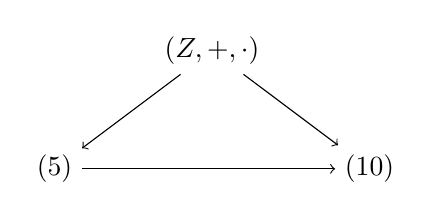
\begin{tikzpicture}
        \node (Z) at (0,0) {$(\mathbb{Z}, +, \cdot)$};
        \node (5) at (-2,-1.5) {$(5)$};
        \node (10) at (2,-1.5) {$(10)$};
        \draw[->] (Z) -- (5);
        \draw[->] (Z) -- (10);
        \draw[->] (5) -- (10);
    \end{tikzpicture}
\end{center}
\noindent
Because
\begin{align*}
    (5) &= \{ 5k : k \in \mathbb{Z} \} = \{ ..., -10, -5, 0, 5, 10, ...\} \\
    (10) &= \{ 10k : k \in \mathbb{Z} \} = \{ ..., -20, -10, 0, 10, 20, ...\}
\end{align*}
\noindent
and $(10) \subseteq (5)$ but $(5)$ is not contained in any other ideal.

\bigskip
\begin{thmBox}{Galois's Theorem on Finite Fields}
    LLet $\mathbb{F}_q$ be a finite field with $q$ elements, then we can only have the following situations:
    \begin{itemize}
        \item $q = p$ where $p$ is a prime number, and in this case $\mathbb{F}_q \simeq \mathbb{Z}_p$, so they are isomorphic.
        \item $q = p^k$ where $p$ is a prime number and $k$ is a positive integer, and in this case $\mathbb{F}_q \simeq \mathbb{F}_p[X] / (f(X))$ where $f(X)$ is an irreducible polynomial of degree $k$ over $\mathbb{F}_p$.
    \end{itemize}
\end{thmBox}

\bigskip

\noindent
\begin{defBox}{Irreducible Polynomial}
    aGiven a field $\mathbb{F}$, a polynomial $f(X) \in \mathbb{F}[X]$ is irreducible if it cannot be factorized into the product of two polynomials of degree >0 and <deg(f(x)).
\end{defBox}

\noindent
\textbf{Remark:}\\
Irreducible polynomials play the same role for polynomials as prime numbers play for integers.
\smallskip

\noindent
Given the ring $(\mathbb{Z}_p[x], +, \cdot)$ all and only the ideal are the sets\\
$(f(x)) = \{ g(x)f(x) : g(x) \in \mathbb{Z}_p[x] \} =$ {multiples of $f(x)$}\\
so, they are the analogue of the ideals $(n)$ for  $\mathbb{Z}$
\medskip

\noindent
If $f(x)$ is irreducible, then $(f(x))$ is a maximal ideal and $\mathbb{Z}_p[X] / (f(x))$ is a finite field with $p^k$ elements, where $k$ is the degree of $f(x)$.
\medskip

\noindent
Indeed, this is the set of classes of equivalence defined by\\
$\forall g_1(x), g_2(x) \in \mathbb{Z}_p[X], g_1(x) \sim g_2(x) \iff g_1(x) + (g_2(x)) \in (f(x)) \iff g_1(x) - g_2(x)  = g(x)f(x)$ for some $g(x) \in \mathbb{Z}_p[X] \iff g_1(x)$ and $g_2(x)$ have the same remainder with respect to the division by $f(x) \iff g_1(x) \equiv g_2(x) \mod f(x)$
\bigskip

\noindent
Thus $\mathbb{Z}_p[X] / (f(x))$ is the set of all possible reminders with respect to the division by $f(x)$, which are polynomials of degree < deg($f(x)$).\\
Indeed, given $h(x) \in \mathbb{Z}_p[X]$, we can write $h(x) = q(x)f(x) + r(x)$ where $r(x)$ is the remainder and $\deg(r(x)) < \deg(f(x))$.\\
\smallskip

\noindent
Thus a reminder, i.e., an element of $\mathbb{Z}_p[X] / (f(x))$, is a polynomial of kind $a_0 + a_1x + \cdots + a_{k-1}x^{k-1}$ where $a_i \in \mathbb{Z}_p$.\\
\smallskip
\noindent
Thus we have $p^k$ possible reminders, this is, $p^k$ possible elements in $\mathbb{Z}_p[X] / (f(x))$.\\


\newpage
\noindent
\textbf{Remark:}\\
Let $\mathbb{F}$ be a field:
\begin{itemize}
    \item if $f(x) \in \mathbb{F}[X]$ has a \underline{root} $\alpha \in \mathbb{F}$ (i.e., $f(\alpha) = 0$), then $f(x)$ is \underline{not} irreducible (it is irreducible). (*)
    \item if $f(x) \in \mathbb{F}[X]$ has degree 2 or 3 and has \underline{no root} in $\mathbb{F}$, then $f(x)$ is irreducible (if $\deg(f(x)) > 3$ and $f$ has no roots, we can not say anything)
\end{itemize}
\noindent
(*) Remember that if $\alpha$ is a root of $f(x)$, then $f(x) = (x - \alpha)g(x)$

\medskip
\begin{propBox}{Irreducibility}
    aA polynomia $f(x) \in \mathbb{Z}_p[X]$ of degree $k$ is irreducible if and only if:
    \begin{itemize}
        \item $f(x) | x^{p^k} - x$
        \item $\forall$ prime $r | k, gcd(f(x), x^{p^{k/r}} - x) = 1$ 
    \end{itemize}
\end{propBox}
\noindent
This proposition works well if $k$ is small (and it can be used very often in the construction of finite fields).\\
In general, it is not efficient  because we need to know the factorization of $k$. But there exist some efficient test for checking the irreducibility of a polynomial.

\noindent\rule{\textwidth}{0.5pt}

\noindent
\paragraph{BIG EXAMPLE: Construction of $\mathbb{F}_4$} 
\noindent
$\mathbb{F}_4 = \mathbb{F}_2$, thus we need to construct $\mathbb{F}_2[X] / (f(X))$ where $f(X)$ is an irreducible polynomial of degree 2 over $\mathbb{F}_2$.
\smallskip

\noindent
Remember that we are working in $\mathbb{F}_2[X]$, thus a polynomial of degree 2 is of the kind $ax^2 + bx + c$ where $a, b, c \in \mathbb{F}_2$.
\smallskip
\noindent
Thus, $a$ can be only equal to $1$ (otherwise the polynomial does not have degree 2)\\
$b, c \in \{0, 1\}$, thus we have 4 possible polynomials of degree 2:
\medskip

\noindent
$x^2, x^2 + 1, x + 1, x^2 + x + 1$
\begin{itemize}
    \item $x^2$ is not irreducible because it has a root (0)
    \item $x^2 + 1 = (x + 1)(x + 1) = (x + 1) ^2$ is not irreducible (1 is a root)
    \item $x^2 + x = x(x + 1)$ is not irreduucible (0 and 1 are roots)
    \item $x^2 + x + 1$ is irreducible (it has no roots in $\mathbb{F}_2$)
\end{itemize}

\medskip

\noindent
Thus $\mathbb{F}_4 = \mathbb{F}_2[X] / (x^2 + x + 1)$ = {reminders with respect to the division by $x^2 + x + 1$} = {all polynomials $\in \mathbb{F}_2[X]$ of degree < 2} = $\{ 0, 1,$ [poly of deg 0] $x, x+1 $[poly of deg 1] $\}$
\smallskip

\noindent
$\mathbb{F}_4 = \{ 0, 1, x, x+1 \} = \{ 0, 1, \alpha, \alpha+1 \}$ where $\alpha$ is a root in $\mathbb{F}_2$ of $x^2 + x + 1$ (somewhere else!)
\bigskip

\noindent
Let us observe that $x$ and $\alpha$ have the same behavior.\\
Indeed, $x^2 + x + 1$  is irreducible in $\mathbb{F}_4$, becasue $x^2 = 1(x^2+x+1) + x + 1$ where 1 is the quotient and $x + 1$ is the reminder.\\
Indeed, $x^2 + x + 1 + x + 1 = x^2 + 2x + 2 = x^2$ because we are working in $\mathbb{F}_2$ and $2x = 0$ and $2 = 0$.
\medskip

\noindent
On the other hand, it is possible to observe that:\\
$x^2 \equiv x^2 + x^2 + x + 1 \mod x^2+x+1 \implies x^2 \equiv 2x^2 + x + 1 \mod x^2 + x + 1 \implies x^2 \equiv x + 1 \mod x^2 + x+ 1$
\smallskip

\noindent
Similarly, since $\alpha$ is a root of $x^2 + x + 1$, we have $\alpha^2 + \alpha + 1 = 0 \implies \alpha^2 = - \alpha - 1 \implies \alpha^2 = \alpha + 1$.

\noindent
\textbf{End example}\\
other practial examples have been provided at lecture of 13-03-2026
\bigskip

\begin{defBox}{Primitive}
    aGiven $f(x) \in \mathbb{F}_p[X]$ if $f(x)$ is irreducible and \\
    $<x> = (\mathbb{F}_p[X]/(f(x)))^2$ then $f(x)$ is called primitive.
\end{defBox}
\bigskip

\begin{thmBox}{Cyclicality of Finite Fields}
    gGiven a finite field $\mathbb{F}_q$, then $(\mathbb{F}_q^x, \cdot)$ is a cyclic group.
\end{thmBox}

\noindent
These concepts are strictly related to the cryptographic applications, and they will be used in the construction of the AES (Advanced Encryption Standard) and in the construction of the elliptic curves.
\medskip

\noindent
For istance, \textbf{AES:}
\\
It is possible see AES consideing the fact that \textit{"bites are strings of bites of lenght 8. The number of possivle bytes is $2^8$"}\\
So $\mathbb{F}_2^8 = \mathbb{F}_2 \cdot \mathbb{F}_2 \cdots \mathbb{F}_2$ (8 times) VECTOR SPACE, but we can also see it as a field, because we can find an irreducible polynomial of degree 8 over $\mathbb{F}_2$, thus we can write\\
$\mathbb{F}_{2^8} = \mathbb{F}_2 [X] / (f(X))$ where $f(X)$ is an irreducible polynomial of degree 8 over $\mathbb{F}_2$.\\
$a_7x^7 + a_6x^6 + \cdots + a_1x + a_0$ where $a_i \in \mathbb{F}_2$ is the representation of a byte in AES (0, 1), and the operations of AES are defined as the operations of $\mathbb{F}_2[X] / (f(X))$.\\
\medskip

\noindent
In AES $\mathbb{F}_{2^8} \simeq \mathbb{F}_2[X] / (x^8 + x^4 + x^3 + x + 1)$ 


\begin{quote}
\textit{\textbf{Author's Note:} The Professor underlined that it is important, during individual study, to consider the difference between the two representations of $\mathbb{F}_{2^8}$, because they are equivalent but they have different properties.\\
In particular, the representation $\mathbb{F}_2^8$ is a vector space, thus it has a basis and we can represent the elements of $\mathbb{F}_{2^8}$ as linear combinations of the basis elements, while the representation $\mathbb{F}_2[X] / (f(X))$ is a field, thus it has a multiplicative structure and we can find the inverse of an element with respect to the multiplication.}
\end{quote}

